\section{vRNIC Design}
To achieve unified RDMA virtualization, we design vRNICs, which is software virtualization with complete RDMA attributes (e.g. QPs). Both conatiners and VMs can use vRNICs through unified drivers. In this section, we firstlly introduce vRNIC virtualization and its driver. Then, optimizations for performance are introduced.

\subsection{vRNIC Virtualization}
To make vRNIC flexible and hardware-independent, we construt each vRNIC in host by software methods. Besides, software methods are more scalable and isolated for VMs or containers.

Moreover, both kernel-space and user-space are feasible to construct vRNICs in host. Compared to kernel-space, there are multiple advantages for vRNICs in user-space, such as minimal attack surface, flexible management and independent on RDMA kernel drivers. Thus, we choose the user-space for vRNIC virtualization.

\subsubsection{Static Attributes} ~\\
In summary, RNIC has two kinds of hardware properties, namely static property and dynamic property: Static attributes mean unchanged and unrecorded attributes in physical RNIC. For example, the device name and resource handle are both static for RNIC. Compared, dynamic attributes means they should be recorded into or generated from hardware exiplictly. For example, QP is dynamic beacause it should to be reflected in RNIC.

For static attributes, we directly use virtual names for them. For example, the device name of vRNIC is virtual. Besides, the address of vRNIC is also virtual. There are two main advantages for these: first, virtual information hids the real hardware informations for clouds' user; second, virtual information, especially virtual address is basic to construct a virtual network. 
\subsubsection{Dynamic Attributes} ~\\
However, for dynamic attributes, the hardware cannot regconize virtual informations. Thus, we need map the so-called virtual dynamic attributes to physical RNIC to make them effective. For example, when application calls post\_send, the vRNICs can drive physical RNIC to transport the corresponding data. Thus, in our design, the vRNIC is flexible for management. 

Fortunately, all RDMA resources information in RNIC are only changed in control path and maintained in data path. So, we can map the virtual RDMA resources to RNIC only in control path, such as QP and Doorbell,  and do not need introduce any operations in data path. Mapped RDMA resources are directly used and RNIC is notified by mapped virtual DoorBell in vRNIC. As a result, vRNIC are still with DMA zero-copy, hardware protocol stack processing and other high-performance capability in data path. Therefore, we put each vRNIC with a map unit. As Figure~\ref{fig:map-unit} shows, it maps or unmaps virtual RDMA resources from vRNIC to RNIC in control path:-


\begin{figure}[!ht]
	\centering
	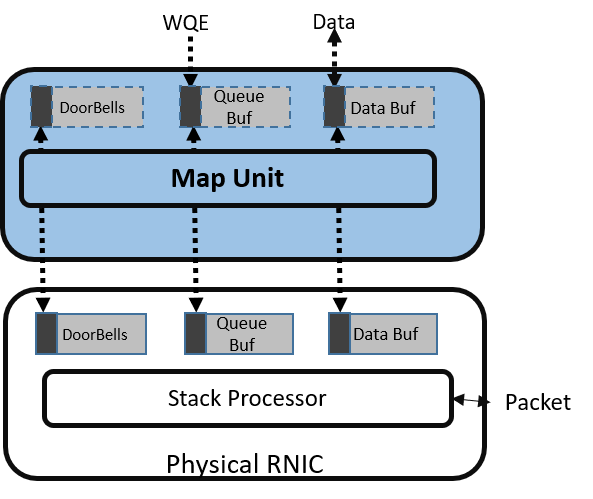
\includegraphics[width=0.9\linewidth]{images/map-unit}
	\caption{Map Unit in vRNIC}
	\label{fig:map-unit}
\end{figure}

For RDMA resources (e.g. QPs, CQs): Taking QP as an example, regularly, vRNIC record virtual RDMA resources information when the virtual QP instance are created. However, virtual QP are still not generated-associated with the RNIC. To make the mapping, the map unit will create corresponding real QP instance in RNIC based on the information of virtual QP instances, such as the same memory address information and the same device id. Equivalently, the virtual QP information are recognized in RNIC, such as QP number and QP state, and can be one-to-one synchronous with RNIC’s physical instance by lots of similar map operations in control path. All operations can be completed by calling the Verbs interface of RNIC in user space. After the mapping is completed, the work requests in the vRNIC virtual QP can be zero-copied into the RNIC. Also, data in registered memory of vRNIC can also be zero-copied to RNIC in the same way. 

For DoorBells: It needs to be mapped to the hardware doorbell in the physical NIC device space, so that vRNIC can notify the RNIC hardware processors. In vRNIC, the mapping unit will map the virtual address of the virtual doorbell to the hardware doorbell address of the corresponding physical NIC device space through a system call. As shown in Figure~\ref{fig:map-unit}, after the mapping is completed, the write operation to the vRNIC virtual doorbell is equivalent to performing the doorbell notification to the RNIC.

Map unit is the key for vRNICs' performance. Note that all mapping relationships are all one-to-one, therefore, the correctness and isolation of resources in different RDMA context are guaranteed. Meanwhile, because the mapping operation is only executed in control path, the overhead is one-off compared to data commands. For the data path, vRNICs can directly utilize the hardware processing capability of RNIC, such as DMA zero-copy and hardware protocol stack processing.

\subsection{Unified vRNIC Driver}
vRNIC is virtual device with complete RDMA attributes. However, vRNICs are still independent software in host user space. Thus, for VMs and containers, the driver (or library in containers) for vRNICs should be designed. Unification is necessrary for vRNIC driver, beacause it hides the difference of applications' environments and makes the centralized management (e.g. the virtual layer in later section) easier.

For containers, vRNICs can be directly provided to RDMA applications in containers with some modification in containers' verbs library. However, vRNICs  and VMs' application are isolated with the hypervisor and guest OS. vRNICs needs to be recongnized by VMs' hypervisor and then provided by guest OS. Thus, the I/O virtualization shoulde be used to extend each vRNIC for VMs. Then, specific driver for vRNICs installed in guest OS. 

However, the main challenge of above is how to make vRNICs unified to all RDMA applications. Thus, the comminucation between vRNIC to VMs or containers must be consistent. To make vRNICs communication consistent, we design a unified protocal from vRNIC to VMs' hypervisor or containers' applications. Note that both containers' applications and VMs are processes for host. Thus, I/O channel between vRNIC and VM is shared memory with specific protocal, e.g. vhost-user. And that is nature to containers' applications. Besides, the notification is used in event descriptor.

The goal of the device driver is to support I/O process inside each guest. As shown in in Figure~\ref{fig:vrnic-driver},  the commands of RDMA application be forwarded into the memory-shared queue, and trigger events to notify the vRNIC to process them; similarly, the device driver receives interrupt notifications and reads the result from vRNIC. In short, the device driver can be implemented by a lightweight kernel module.

\begin{figure}[!ht]
\centering
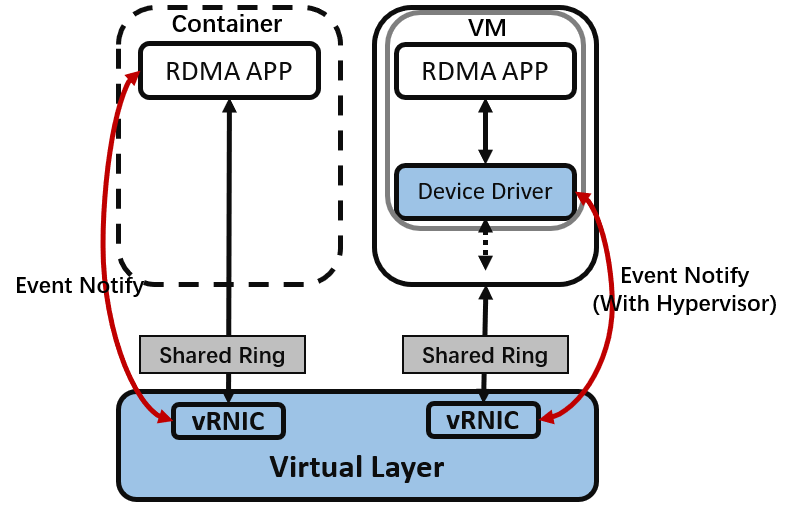
\includegraphics[width=1.0\linewidth]{images/interface-general}
\caption{Unified vRNIC Driver}
\label{fig:vrnic-driver}
\end{figure}

	
\subsection{Performance Optimization}
Trough vRNIC driver, all commands of RDMA applications can be excuted in vRNICs. However, in data path of vRNIC, there is still data-copy. Also, the data commands are forwarded to vRNIC for execution. These brings the data-copy or context-switch latency for RDMA applications. 

To address above performance problems, we map RDMA resources between vRNICs and appications. However, there are two different RDMA resources for vRNICs: resources in host physical memory (such as QPs, MRs), resources in physhical RNIC (e.g. DoorBell registers). 

(1) For QPs or MRs: The fact of zero-copy is that both processes have common available physical memory pages. Same as native RDMA, the zero-copy contents are including the RDMA work request in QPs and data in MRs. 
Similar as the above I/O channels, we use shared memory to map applications' memroy to vRNICs' RDMA resources (e.g. QPs and MRs). And this mapping is feasible for both VMs and containers.

\begin{figure}[!ht]
	\centering
	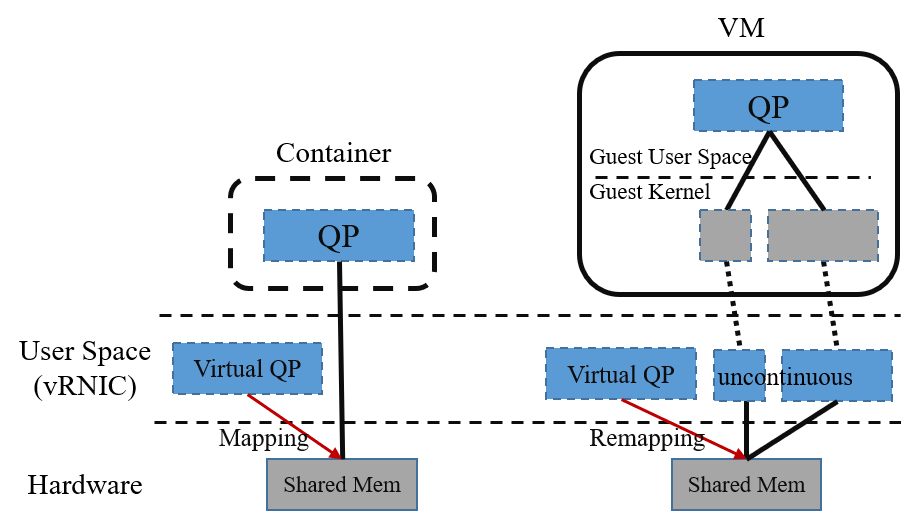
\includegraphics[width=1.0\linewidth]{images/zero-copy}
	\caption{Mapping QP to vRNIC}
	\label{fig:zero-copy}
\end{figure}

However, in the virtual machine, due to the memory management mechanism of guest operating system, the virtual machine's physical memory of the RDMA resource may be not continuous, and the mapped memory area in vRNIC is not continuous like Figure~\ref{fig:zero-copy}. So, vRNIC cannot map the virtual memory area as a virtual RDMA resource to RNIC. To solve this problem, the virtual memory remapping mechanism in user space is used. It remaps the discontinuous RDMA resource virtual memory area in vRNIC to the a block of continuous virtual memory, and the sequence of mapped physical memory page must be unchanged.

(2) For doorbells: Pressing the doorbell is necessary in RDMA data path to drive RNIC. In vRNIC, the doorbell that is mapped to physical RNIC, still need to be mapped to RDMA application to meet bypassing. Otherwise, the pressing command needs be forward to vRNIC and that’s imports apparent latency in data path.

However, the RDMA application and the vRNIC belong to two different processes on the host, and they have isolated virtual address spaces. At the same time, the doorbell register is in the device address space and cannot be mapped by shared memory. The key to solving this problem is that the process of RDMA application needs to know the physical address of the doorbell register.

\begin{figure}[!ht]
	\centering
	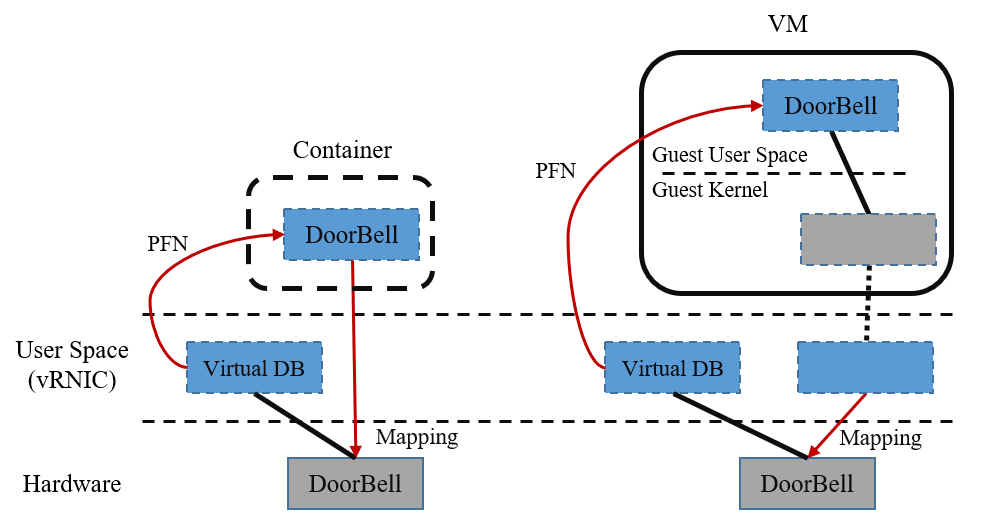
\includegraphics[width=1.0\linewidth]{images/by-pass}
	\caption{Mapping DB from vRNIC}
	\label{fig:by-pass}
\end{figure}

Therefore, when an RDMA application creates a RDMA context, as shown in Figure~\ref{fig:by-pass}, it sends a request to the vRNIC at first. Under the supervision of virtual layer, vRNIC forwarded to application with the corresponding physical address of the doorbell, commonly the physical page number. After that, the application maps its doorbell virtual address to the physical page in its own process, that needs the host kernel and hypervisor if the application in virtual machines.

